% \documentclass[a4paper,10pt]{article}
\documentclass[a4paper,8pt]{extarticle}
\usepackage{eurosym}
\usepackage[utf8]{inputenc}
\usepackage[T1]{fontenc}
\usepackage{lmodern}
\usepackage{graphicx}
\usepackage{background}
% \usepackage[paperheight=16in,paperwidth=8in,margin=1in,heightrounded]{geometry}
\usepackage[a4paper, width=5.5in, top=0.85in, bottom=0.8in]{geometry}
\usepackage[english,ngerman]{babel}
\usepackage{anyfontsize}
\usepackage{fancyhdr}
\usepackage{textcomp}


% uncomment for htlatex
% \providecommand{\pgfsyspdfmark}[3]{}
% \renewcommand{\includegraphics}[2][]{}
% \renewcommand{\textcolor}[2][]{}


\pagestyle{fancy}
\fancyhf{}
\cfoot{Download: https://github.com/0x0000000001/symmetrielizenz}
\renewcommand{\headrule}{}


\renewcommand{\familydefault}{\sfdefault}
\setlength{\parindent}{0pt}
\setlength{\parskip}{0.8\baselineskip}
\pagenumbering{gobble}
\pdfsuppresswarningpagegroup=1


% \title{\vspace{-1.1cm}\raisebox{-4mm}{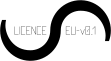
\includegraphics[width=2.0cm]{img/s.pdf}}\ \ Symmetrielizenz / Symmetry Licence\ \ EU-v0.1}
\author{}
\date{}

\pdfinfo{%
  /Title    (Symmetrielizenz / Symmetry Licence - EU-v0.1)
  /Author   (0x01)
  /Creator  ()
  /Producer ()
  /Subject  ()
  /Keywords (Symmetrie Kompensation Ausgleich Lizenz Symmetrielizenz Symmetry Compensation Licence)
}


\backgroundsetup{contents={}}
\begin{document}
% \eject \pdfpageheight=10.5in
\selectlanguage{ngerman} \shorthandoff{"}
\frenchspacing
% \nonfrenchspacing
\fontsize{8.1pt}{9pt}\selectfont

% \maketitle
\begingroup
  \centering
  \LARGE \raisebox{-4mm}{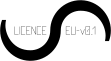
\includegraphics[width=2.0cm]{img/s.pdf}}\ \ Symmetrielizenz / Symmetry Licence\ \ EU-v0.1\\[3em]
\endgroup


Während der Debatte zur neuen EU-Urheberrechtsrichtlinie wurde deutlich, dass es Medienkonzernen möglich ist, die EU-Politik bzw. Gesetzgebung zu kontrollieren. Durch diese Urheberrechtsrichtlinie können die Medienkonzerne nun ohne Gegenleistung und ohne weiterer staatlicher Kontrolle europaweit Menschen ausbeuten und jegliche öffentliche Kommunikation in sozialen Netzen zensieren. Dies trifft dabei genau diejenigen, die zwar keinem Label oder Verlag angehören, die jedoch einen Großteil der Schaffenshöhe und einen wichtigen Anteil im unter anderem politischen Diskurs im Internet erbringen.

Daher erscheint es sinnvoll, möglichst viele selbst erstellte Werke (außer dieses) unter eine Lizenz zu stellen, die EU-Medienkonzerne bei deren Bereicherung an fremder Arbeit zumindest etwas zum Überlegen zwingt und mit Glück auf Probleme in der EU-Urheberrechtsrichtlinie aufmerksam macht.

\emph{Werke, die auf herkömmliche Presse angewiesen sind, sollten nicht unter diese Lizenz gestellt werden.}

Die Idee dahinter ist, die gleichen, leider nicht sehr fairen, Prinzipien wie Artikel 13/17 der neuen EU-Urheber\-rechts\-richt\-linie zu verwenden, nur diesmal gegen die Seite der Verlage. Die beanstandeten Prinzipen in der EU-Urheber\-rechts\-richt\-linie sind
\begin{itemize}
 \item das Verbot der Verwendung selbst kleiner Ausschnitte geschützten Materials, auch für Privatgebrauch wie soziale Online-Interaktionen und zudem
 \item die Sippenhaftung - die Haftung von sozialen Kommunikationsplattformen für Urheberrechtsverstöße von Benutzern.
\end{itemize}

Zudem geht es in dieser EU-"Urheber\-rechts"-richt\-linie nicht einmal um die Rechte der Urheber, sondern die der Verlage. Durch diese Lizenz sollen daher auch ausschließlich Verlage Lizenzgebühren zahlen, die Geld aufgrund der neuen EU-Urheber\-rechts\-richt\-linie eintreiben. Sobald eine ihrer Zeitungen oder sonstigen Unternehmen eines der dadurch geschützten Werke "raubkopiert", müssen die Verlage die vollen Lizenzkosten quasi als Ausgleich zahlen. Alle Anderen dürfen die geschützten Werke weiterhin verwenden.

Das Ziel ist, möglichst viele Videos, Texte, Fensterbilder und was auch immer geht, unter diese Lizenz zu stellen. Eventuell auch Graffitis, dann werden sogar von deren Reporter geschossene Fotos zu "Raubfotos".

Dies alles soll für ein Bewusstsein sorgen, welche Probleme die neue EU-Urheberrechtsrichtlinie heraufbeschwört.

Einer der wichtigen Punkte der Lizenz ist, das Eintreiben der Gebühren jedem zu erlauben und dafür einen Teil der Lizenzkosten abzutreten. Dadurch können sich Menschen finden, die beruflich die entsprechenden Verlage auf Verstöße durchsuchen und Sammelklagen durchführen. Das mag schmutzig wirken, aber es soll vor allem die "Klagearbeit" vom kleinen Künstler weg bringen, zu Menschen die sich das Risiko leisten können oder wollen, sich mit skrupellosen Konzernen vor Gericht zu duellieren.

Auf den nächsten Seiten folgt der Lizenztext. Ich gebe ihn ohne Einschränkungen für jegliche Verwendung frei. Ich bin kein Jurist, daher weiß ich nicht ob alle darin aufgeführten Bedingungen überhaupt rechtlich durchsetzbar sind. Ich weiß nicht einmal ob dies eine gute Idee ist, aber bevor ich gar nichts mache, versuche ich es zumindest.

Wenn sich jemand rechtlich auskennt, wäre ich natürlich immer für Hinweise dankbar.

\ 

{\small PS:

Ein Ausblick auf momentan bearbeitete Gesetze zeigt, wohin wir uns bewegen. Die zunehmende Macht der Medienkonzerne gegenüber Politik und Bevölkerung ist bereits jetzt ein gewaltiges Problem. Sie kontrollieren bereits offensichtlich die Meinung der Massen durch deren Monopol auf Nachrichten in Form von Zeitungen, Radio und Fernsehen. Offenbar reicht dies bereits, zusätzlich möglicherweise mit Bestechung bzw.\ Lobbyisten, um Politik bzw.\ Gesetzgebung zu kontrollieren (siehe die Diskussion zur EU-Urheberrechtsrichtlinie). Da Menschen in der Masse ähnlich sind, funktioniert diese Art der Manipulation auch bei Polizei und Militär. Dadurch kontrollieren diese Konzerne bereits alles, das durch die Gewaltenteilung einmal gesetzlich getrennt wurde. Also Gesetzgebung (Legislative), ausführende Gewalt (Exekutive) und Rechtsprechung (Judikative). Als zusätzliches Mittel verfügen die Medienkonzerne in Zukunft über einen vollständig kontrollierten, beliebig parteiischen Informationsstrom, an dem es kein Vorbei gibt. Dabei ist die neue EU-Urheberrechtsrichtlinie essentiell, die es den Medienkonzernen erlaubt, jegliche reichweitenwirksame Veröffentlichung von Vorfällen, konträren Meinungen und vor allem jegliche Organisation zum Widerstand im Keim zu blockieren. Denn es handelt sich dabei um eine vorgeblich zwecks "Urheberrechtsschutz" eingeführte Zensur-Infrastruktur in deren Händen und ohne richterlicher oder polizeilicher Kontrolle. Zusätzlich werden momentan Gesetze entworfen oder bereits erlassen, die es verbieten, Passwörter für Online-Kontos geheim zu halten und überhaupt anonym zu kommunizieren (siehe IT-Sicherheitsgesetz in DE). Außerdem wird versucht, das Trennungsgebot zwischen Nachrichtendiensten und Polizei zu entfernen (ebenfalls in DE). Ein weiterer Punkt sind die Nachrichtendienste selbst, die über das neue Geheimdienstermächtigungsgesetz die Erlaubnis erhalten, in Wohnungen im Inland einzubrechen und dort Wanzen und Trojaner zu installieren, natürlich auch bei den eigenen Staatsbürgern (ebenfalls in DE). Diese ganzen Gesetze und Richtlinien wurden bereits länger geplant und vorbereitet. Sie werden jedoch momentan alle in einem extrem kurzem Zeitraum erlassen und in zwei Jahren volle Wirksamkeit erlangen. Einen derartigen Vorstoß hat es bisher das letzte Mal im Jahr 1933 mit dem Ermächtigungsgesetz gegeben.

Auch wenn wir von Medienkonzernen regiert werden, werden wir Kriege gegen andere Länder führen.\\
Wir werden es dann sogar wollen.}


\pagebreak
% \eject \pdfpageheight=15in
\setlength{\parskip}{0.5\baselineskip}

\backgroundsetup{
scale=1,
color=black,
opacity=0.2,
angle=0,
contents={%
  
\includegraphics[width=0.8\textwidth]{img/justitia.pdf}
  }%
}

\section{DE: Symmetrielizenz EU-v0.1}
\label{DE}

Es gleicht einer Enteignung, wenn Millionen Menschen Inhalte produzieren, diese auf Plattformen sozialer Kommunikation im Internet publizieren und zumeist kein Geld dafür erhalten, aber stattdessen Contentverwalter von den Plattformen allgemeine Gebühren verlangen dürfen, da die in der Richtlinie (EU) 2019/CopyrightSingleMarket als Alternative angebotenen Filter nicht in der notwendigen Qualität implementierbar sind.

\begin{enumerate}
 \item Als Ausgleich und da hauptsächlich Contentverwerter damit Geld verdienen, darf jeder außer Contentverwerter, das unter dieser Lizenz stehende Werk gebührenfrei verwenden, verändern und weiter geben, solange das Ergebnis unter dieser Lizenz bleibt.

 \item \label{DEcosts} Contentverwerter dürfen dieses Werk ebenfalls verwenden, verändern und weiter geben, solange dies im Rahmen dieser Lizenz geschieht. Sie haben jedoch für jede nicht mit den beteiligten Autoren vereinbarte Verwendung den monetären Gegenwert von 20 kg Gold an den ursprünglichen Autor und jeweils den monetären Gegenwert von 0,25 kg Gold an jeden beteiligten Autor an Lizenzgebühren zu zahlen.
 
 Sind diese fixen Lizenzgebühren nicht rechtlich zulässig, werden sie durch eine variable Gebühr ersetzt, wobei für jeden beteiligten Autor der an ihn zu zahlende Lizenzbetrag einzeln durch den "monetären Gegenwert von 0,005 kg Gold", mal "der Arbeitszeit des einzelnen beteiligten Autors am Werk in Stunden, aufgerundet auf volle Stunden", mal "der Anzahl der von der Veröffentlichung (auch in Zukunft) erreichten Personen", zu bestimmen ist. Liegt keine unbestreitbare Personenzahl vor, wird ein Fünftel der Gesamtzahl der Personen verwendet, die der einzelne technische Kommunikationskanal (z.B.\ Fernsehsender oder Zeitung) des veröffentlichenden Contentverwerters erreicht.

 \item Eine anteilsmäßige Lizenzgebühr gilt für Ausschnitte bzw.\ Teile, auch wenn diese verändert wurden, und ebenfalls für Zitate aus dem Werk unter dieser Lizenz.

 \item Contentverwerter können mit den beteiligten Autoren niedrigere Lizenzgebühren für ein Werk vereinbaren, allerdings nur vor dessen Verwendung.

 \item Der "ursprüngliche Autor" ist im Rahmen dieser Lizenz die natürliche Person oder Personengruppe, die initial das Werk erstellt hat.

 \item Ein "beteiligter Autor" ist im Rahmen dieser Lizenz der ursprüngliche Autor und jede aktiv an der Schaffung des Werkes beteiligte natürliche Person. Dies kann auch eine natürliche Person sein, die das Werk in weiterer Folge bearbeitet hat. Ein beteiligter Autor ist nur dann ein beteiligter Autor, wenn noch Anteile der Leistung im verwendeten Werk enthalten sind.

 \item Die "Richtlinie (EU) 2019/CopyrightSingleMarket" ist im Rahmen dieser Lizenz die "Richtlinie (EU) .../2019 des Europäischen Parlaments und des Rates vom ... über das Urheberrecht und die verwandten Schutzrechte im digitalen Binnenmarkt und zur Änderung der Richtlinien 96/9/EG und 2001/29/EG" und alle davon abgeleiteten Gesetze und Richtlinien.

%  \item "Plattformen sozialer Kommunikation im Internet" sind im Rahmen dieser Lizenz "Diensteanbieter für das Teilen von Online-Inhalten" laut Abschnitt 2(6) der Richtlinie (EU) 2019/CopyrightSingleMarket.
 
 \item "Contentverwalter" sind im Rahmen dieser Lizenz juristische Personen, die Gebühren laut Richtlinie (EU) 2019/CopyrightSingleMarket einfordern und deren Jahresumsatz 10 Millionen \euro\ übersteigt.

 \item "Contentverwerter" sind im Rahmen dieser Lizenz der Contentverwalter und zusätzlich alle von diesem beauftragte juristische Personen. Dazu gehören auch durch beauftragte und indirekt beauftragte juristische Personen beauftragte juristische Personen, also indirekt beauftragte juristische Personen beliebiger Tiefe.

 \item Für die Lizenzgebühren dieser Lizenz muss immer der Contentverwalter aufkommen, der den Lizenzverstoß selbst oder durch beauftragte natürliche oder juristische Personen beliebiger Tiefe begangen hat.
 
 Falls dies nicht rechtlich zulässig ist, hat die oberste beauftragte juristische Personen zu zahlen, bei der dies rechtlich zulässig ist und die den Lizenzverstoß selbst oder durch beauftragte natürliche oder juristische Personen beliebiger Tiefe begangen hat. Natürliche Personen sind von der Lizenzzahlungspflicht befreit.

 \item Lizenzgebühren können von jedem außer Contentverwerter eingefordert und eingeklagt werden, sobald eine Lizenzverletzung vorliegt.

 \item Wer die Lizenzgebühren erfolgreich geltend macht, kann 30 \% der Lizenzgebühren einbehalten, nur die übrigen 70 \% müssen an die beteiligten Autoren anteilsmäßig weiter gezahlt werden. Das früheste Datum einer Lizenzforderung bestimmt, wer die Lizenzen einfordert und verteilt. Verzögert dieser die Forderung ungebührlich, so kann ein anderer die Einforderung der Lizenzgebühren übernehmen.

 \item Lizenzgebühren können pro Veröffentlichung nur einmal erfolgreich eingefordert werden. Das mehrfache Ausliefern eines bestimmten Werkes unter dieser Lizenz an mehrere Benutzer oder Kunden zählt nicht als mehrfache Veröffentlichung.

 \item Jegliche weitere Verwendung, Veränderung und auch jeder Ausschnitt oder Teil eines Werkes unter dieser Lizenz, steht ebenfalls immer unter dieser Lizenz. Dies inkludiert auch Zitate.
 
 \item Diese Lizenz kann in Kombination mit anderen Lizenzen verwendet werden, dabei gelten die Lizenzen parallel. Eine Erlaubnis einer Lizenz kann dabei die Einschränkungen oder Forderungen einer anderen Lizenz nicht abschwächen. Es gilt somit die Vereinigungsmenge der Einschränkungen bzw.\ Forderungen und die Schnittmenge der Erlaubnisse aller Lizenzen.

 \item Sollten Sätze oder Wörter dieser Lizenz ungültig sein, bleibt die übrige Lizenz gültig. Die grundsätzliche Bedeutung dieser Lizenz darf dadurch allerdings nicht in extremer Weise geändert sein.

 \item Dieser Lizenztext samt Bilder darf von jedem frei veröffentlicht und verwendet werden.
\end{enumerate}

\begin{center}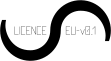
\includegraphics[width=0.7cm]{img/s.pdf}\end{center}


\pagebreak
\selectlanguage{english} \shorthandoff{"}
\frenchspacing
% \nonfrenchspacing
\section{EN: Symmetry Licence EU-v0.1}
\label{EN}

It is akin to expropriation when millions of people produce content, publish it on social communication platforms on the internet, usually without receiving money for it, but instead of them content managers are allowed to charge the platforms for general fees, as the filters offered in Directive (EU) 2019/CopyrightSingleMarket can not be implemented with the necessary quality.

\begin{enumerate}
 \item In return and because mainly content utilizers make money with it, anyone other than content utilizers may use, modify and redistribute the work under this licence for free, as long as the result remains under this licence.

 \item \label{ENcosts} Content utilizers may also use, modify and redistribute this work as long as it is done so under this licence. However, they are required to pay the monetary equivalent of 20 kg of gold to the original author and in addition the monetary equivalent of 0.25 kg of gold to each one of the contributing authors in licence fees for any use, not agreed with the contributing authors.
 
 If these fixed licence fees are not legally permissible, they are replaced by a variable fee, with the licence fee payable to each individual contributing author being determined by the "monetary equivalent of 0.005 kg of gold", times "the working time of the individual contributing author on the work under this licence in hours, rounded up to full hours", times "the number of persons reached by the publication (also in the future)". If that number of persons is not indisputable, one fifth of the total number of persons reached by the single technical communication channel (e.g.\ TV channel or newspaper) of the publishing content utilizer will be used.

 \item A pro-rata licence fee applies to excerpts and parts, even when they are modified, and also to quotations from the work under this licence.

 \item Content utilizers can agree lower licence fees for a work with the contributing authors, but only in advance of a use.

 \item The "original author" within the scope of this licence is the natural person or group of natural persons who initially created the work.

 \item A "contributing author" within the scope of this licence is the original author and any natural person who was actively involved in the creation of the work. This may also be a natural person who has subsequently processed the work. A contributing author is only a contributing author, when a portion of the modification or involvement is still included in the work used.

 \item The "Directive (EU) 2019/CopyrightSingleMarket" within the scope of this licence is the "Directive (EU) 2019/... of the European Parliament and of the Council of ... on copyright and related rights in the Digital Single Market and amending Directives 96/9/EC and 2001/29/EC" and all derived laws and directives.

%  \item "Social communication platforms on the internet" within the scope of this licence are "online content-sharing service provider" as defined in Article 2(6) of the Directive (EU) 2019/CopyrightSingleMarket.

 \item "Content managers" within the scope of this licence are juridical persons that demand licence fees under the Directive (EU) 2019/CopyrightSingleMarket and whose annual turnover exceeds \euro\ 10 million.

 \item "Content utilizers" are the content manager and additionally all juridical persons commissioned by the latter. This also includes juridical persons commissioned by commissioned and indirectly commissioned juridical persons, so indirectly commissioned juridical persons of any depth.

 \item The licence fees for this licence must always be paid by the content manager who committed the licence infringement itself or by commissioned natural or juridical persons of any depth.
 
 If this is not legally permissible, the top-level commissioned juridical person has to pay, for which this is legally permissible and which committed the licence infringement itself or by commissioned natural or juridical persons of any depth. Natural persons are exempted from the licence payment obligation.

 \item Licence fees may be claimed by anyone except content utilizers, as soon as there is a licence violation.

 \item Whoever successfully claims the licence fees, may retain 30 \% of the licence fees, and only the remaining 70 \% must be paid pro rata to the contributing authors. The earliest date of a licence claim determines who claims and distributes the licences. If the claim gets delayed improperly by the claiming party, then another one can take over to claim the licence fees.

 \item Licence fees can only be successfully claimed once per publication. The multiple delivery of a particular work under this licence to multiple users or customers does not count as multiple publications.

 \item Any further use, modification and any excerpt or part of a work under this licence is also always under this licence. This also includes quotations.

 \item This licence can be used in combination with other licences, whereby the licences apply in parallel. A permission of a licence cannot weaken the limitations or demands of another licence. Thus, the union of the restrictions or demands and the intersection of the permissions of all licences apply.

 \item If sentences or words of this licence are invalid, the remaining licence remains valid. However, the fundamental meaning of this licence must not be changed in an extreme way by this.

 \item This licence text and images can be freely published and used by anyone.
\end{enumerate}

\begin{center}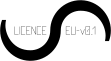
\includegraphics[width=0.7cm]{img/s.pdf}\end{center}

\end{document}
